\documentclass[oneside, 10pt, notitlepage]{book}
	
	
\usepackage{../_mypackages/monographpreamble}
\usepackage{../_mypackages/commands}

\title{Special Relativity} % \MyTitle
\author{Bruno Murino} % \MyAuthor
\date{\today} % \MyDate

\usepackage{../_mypackages/monographstyle}

\graphicspath{ {figures/} }

%--------------------------------------------------------------------------------------------------

\begin{document}
\chapter{Lista XIV}

\section*{Ex. 2)}
Two objects with the same mass \(m\) and speed \(v\) frontally collide inelastically forming a composite object with mass \(M\) and speed \(v'\). We can determine \(M\).

First, let everything happen along the \(x\)-axis, so the momentum and energy conservation reads
\begin{equation}
\begin{split}
    \gamma(v)\ m v + \gamma(-v)\ m(-v) &= \gamma(v')\ M v' \\
    \gamma(v)\  m c^2 + \gamma(-v)\ m c^2 &= \gamma(v')\ M c^2
\end{split}
\end{equation}
Since \(\gamma(v)=\gamma(-v)\), from momentum conservation we see that \(\gamma(v')\ M v'=0\), but the mass is not zero and \(\gamma \geq 1\), so it can only be that \(v'=0\), thus \(\gamma(v')=\gamma(0)=1\), implying that energy conservation means
\begin{equation}
    2\gamma(v)\ m = M
\end{equation}

If \(v = 12c/13\), then \(\gamma(v) = 13/5\) and 
\begin{equation}
    M = \frac{26}{5}m
\end{equation}

\section*{Ex. 3)}

\begin{figure}[H]
    \centering
    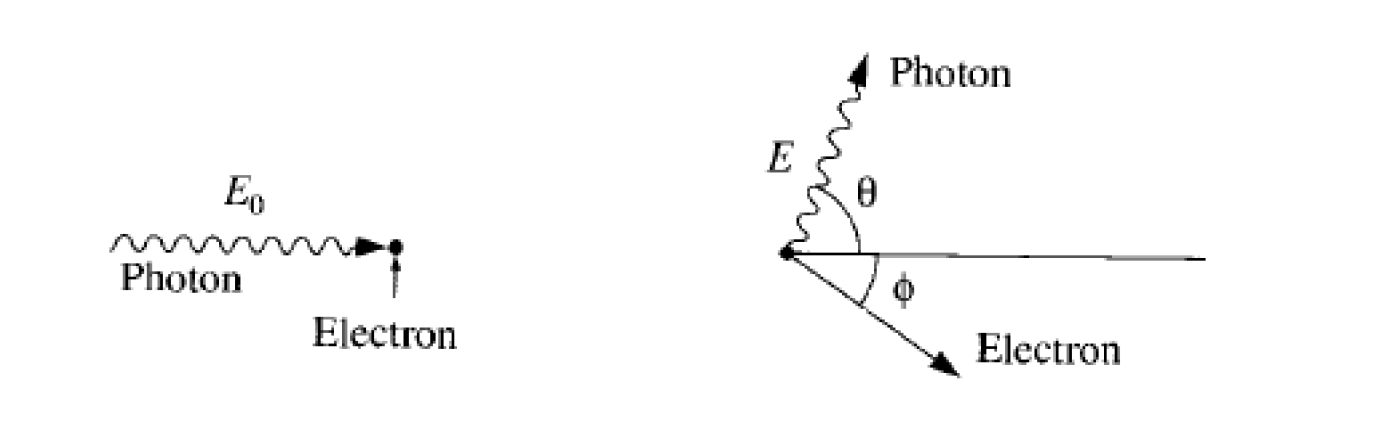
\includegraphics[width=0.7\textwidth]{L14_3}
    \caption{Collision between photon and stationary electron.}
    \label{fig:L14_3}
\end{figure}

We want to find the new wavelength \(\lambda\) of the photon after the collision in terms of \(\lambda_0\) and \(\theta\).

First, lets state the following photon property
\begin{equation}
    E = p c = \frac{hc}{\lambda}
\end{equation}
Now, lets write the momentum and energy conservation
\begin{equation}
\begin{split}
    \vb{p}_0 &= \vb{p}+\vb{p}_e \\
    E_0 + m c^2 &= E + E_e
\end{split}
\end{equation}
where \(\vb{p}_0\) is the initial momentum of the photon, \(\vb{p}\) is the momentum of the photon after the collision, \(E_e\) is the energy of the electron after the collision and \(\vb{p}_e\) is the momentum of the electron after the collision, and 
\begin{equation}
    E_e = \sqrt{p_e^2 c^2 + m^2 c^4}
\end{equation}

Conservation of energy yields
\begin{equation}
    p_0 c + mc^2 = p c + \sqrt{p_e^2 c^2 + m^2 c^4}
\end{equation}
so
\begin{equation}
    (p_0-p) + mc = \sqrt{p_e^2  + m^2 c^2}
\end{equation}
and 
\begin{equation}
    m^2 c^2 + 2(p_0 - p)mc + \lr{p_0 - p}^2 = p_e^2  + m^2 c^2
\end{equation}
thus 
\begin{equation}
    p_e^2 = 2(p_0 - p)mc + \lr{p_0 - p}^2  
\end{equation}
and finally 
\begin{equation}\label{eq:peen}
    p_e^2 = p_0^2 + p^2 - 2p_0p + 2(p_0 - p)mc
\end{equation}
While conservation of momentum yields 
\begin{equation}\label{eq:pemom}
\begin{split}
    \vb{p}_e &= \vb{p}_0 - \vb{p} \\ 
    p_e^2 &= p_0^2 + p^2 - 2 p_0 p \cos \theta
\end{split}
\end{equation}
Plugging \eqref{eq:pemom} on \eqref{eq:peen} we eliminate \(p_e^2\) and find
\begin{equation} 
\begin{split}
    p_0^2 + p^2 - 2p_0p + 2(p_0 - p)mc &= p_0^2 + p^2 - 2 p_0 p \cos \theta \\
    p_0p - (p_0 - p)mc &=   p_0 p \cos \theta \\
    mc(p_0 - p) &= p_0 p \lr{1-\cos\theta} \\
    mc \lr{\frac{p_0-p}{p_0 p}} &= 1-\cos\theta \\
    mc \lr{\frac{1}{p}-\frac{1}{p_0}} &= 1- \cos\theta
\end{split}
\end{equation}
And recalling that \(\lambda = h/p\), follows \(1/p = \lambda/h\), then 
\begin{equation}
    \frac{mc}{h} \lr{\lambda-\lambda_0} = 1- \cos\theta
\end{equation}
thus 
\begin{equation}
    \lambda = \lambda_0 + \frac{h}{mc}\lr{1-\cos\theta}
\end{equation}

\section*{Ex. 4)}

Before the collision, there is one proton moving with momentum \(\vb{p}\), and one at rest. After the collision there are three protons and one antiproton, all moving with total momentum \(\vb{p}'\). 

Let \(S\) be a frame in which there's on proton at rest before the collision, and let \(S'\) be the centre of mass frame. Since \(p^{\mu}p_{\mu}\) is invariant under Lorentz transformation, we can write
\begin{equation}\label{eq:inva}
    E^2 - c^2\vb{p}^2 = E_{cm}^2 - c^2\vb{p}_{cm}^2
\end{equation} 
But, if we are on the centre of mass frame, the centre of mass is not moving! Thus \(\vb{p}_{cm}=0\). Notice that the particles still move, only the \emph{total} momentum of the centre of mass must be zero. 

Before the collision, on frame \(S\), the energy is 
\begin{equation}
    E = mc^2 + E_in
\end{equation}
where \(m\) is the rest mass of the proton and \(E_{in}\) is the energy of the incoming proton. Before the collision, on frame \(S\), the total momentum is just the momentum of the incoming proton, thus 
\begin{equation}
    \vb{p} = \vb{p}_{in}
\end{equation}
Thus, \eqref{eq:inva} becomes 
\begin{equation}\label{eq:ecmt}
    E_{cm}^2 = \lr{mc^2 + E_in}^2 - c^2 p_{in}^2 = \lr{mc^2}^2 + E_{in}^2 + 2 E_{in}mc^2 - c^2 p_{in}^2
\end{equation}
but the energy of the incoming proton satisfy
\begin{equation}
    E^2_{in} = \lr{mc^2}^2 + c^2 p_{in}^2
\end{equation}
thus 
\begin{equation}\label{eq:cpin}
    c^2 p_{in}^2 = E^2_{in} - \lr{mc^2}^2
\end{equation}
Now, plugging \eqref{eq:cpin} on \eqref{eq:ecmt}, we find
\begin{equation}
    E_{cm}^2 = \lr{mc^2}^2 + E_{in}^2 + 2 E_{in}mc^2 - E^2_{in} + \lr{mc^2}^2 = 2\lr{mc^2}^2 + 2 E_{in}mc^2
\end{equation}
then we can write 
\begin{equation}\label{eq:ein}
    E_{in} = \frac{E_{cm}^2 - 2\lr{mc^2}^2}{2mc^2}
\end{equation}
The minimun energy required to produce the antiproton, \emph{only produces the antiproton, it doesn't make it move nor the other three protons}. In this case, after the collision, the four particles are not moving, thus the energy of the system, with respect to the centre of mass frame \(S'\), is simply 
\begin{equation}
    E_{cm} = 4mc^2
\end{equation}
the sum of the four rest energies. Plugging this result on \eqref{eq:ein}, \(E_{in}\) becomes \(E_{in_{min}}\) and 
\begin{equation}
    E_{in_{min}} = \frac{\lr{4mc^2}^2 - 2\lr{mc^2}^2}{2mc^2} = 8mc^2 - mc^2
\end{equation}
thus, the minimum energy the incoming proton needs to produce an antiproton is 
\begin{equation}
    E_{in_{min}} = 7mc^2
\end{equation}
















\section*{Ex. 9)}

\begin{figure}[H]
    \centering
    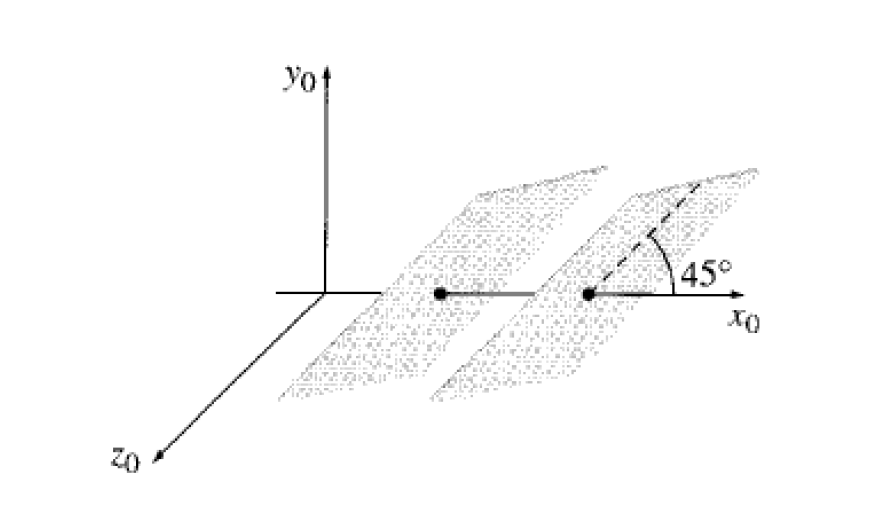
\includegraphics[width = 0.7 \textwidth]{L14_9}
    \caption{Parallel plates, positive to the right and negative to the left.}
    \label{fig:L14_9}
\end{figure}

\subsection*{(a)}

We know that the electric field between parallel plates of surface charge \(\sigma\) points along the normal \(\vu{n}\) from the positive surface to the negative surface and has magnitude \(\sigma/\epsilon_0\)
\begin{equation}
    \vb{E} = \frac{\sigma}{\epsilon_0}\vu{n}
\end{equation}
From figure \ref{fig:L14_9} we can see that
\begin{equation}
    \vu{n} = \frac{-\vu{x}+\vu{y}}{\sqrt{2}}
\end{equation}
thus the field is
\begin{equation}
    \vb{E} = \frac{\sigma}{\epsilon_0\sqrt{2}}\lr{-\vu{x}+\vu{y}}
\end{equation}
Also, there is no magnetic field. 

\subsection*{(b)}
Lets call the frame where the plates are at rest \(S\). Consider a frame \(S'\) moving along the \(x\)-axis to the right, then \(\vb{v}=v\vu{x}\). Recalling how the electric field transforms with a boost along the \(x\)-axis when there's no magnetic field at rest
\begin{equation}
\begin{split}
    E'_x &= E_x \\
    E'_y &= \gamma E_y \\
    E'_z &= \gamma E_z
\end{split}
\end{equation}
Of course \(E_z=E'_z=0\), and only the \(y\) component changes my a factor \(\gamma\), so
\begin{equation}
    E'_x = -\frac{\sigma}{\epsilon_0\sqrt{2}}\vu{x}
\end{equation}
and
\begin{equation}
    E'_y = \gamma \frac{\sigma}{\epsilon_0\sqrt{2}} \vu{y}
\end{equation}
so 
\begin{equation}
    \vb{E}' = \frac{\sigma}{\epsilon_0\sqrt{2}}\lr{-\vu{x}+\gamma\vu{y}}
\end{equation}
Notice that these is the field seen by \(S'\), written using the coordinates of \(S\). Also notice that the unit vector of this field is not \(\lr{-\vu{x}+\vu{y}}/\sqrt{2}\) anymore, it is 
\begin{equation}
    \frac{\lr{-\vu{x}+\gamma\vu{y}}}{\sqrt{1+\gamma^2}}
\end{equation}

\subsection*{(c)}
We already know that the tangent of the angle the object makes with the \(x\)-axis with respect to \(S\), at rest, and \(S'\), boost along \(x\)-axis, relate as
\begin{equation}
    \tan \theta' = \gamma \tan \theta
\end{equation}
So if \(\theta=45^{\circ}\) , \(\tan 45^{\circ} = 1\) and then \(\theta'\) is
\begin{equation}
    \theta' = \arctan \gamma
\end{equation}
So this is the angle the plates make with the \(x\)-axis.

\subsection*{(d)}

The new normal vector is 
\begin{equation}
    \vu{n}' = -\vu{x}\sin\theta' + \vu{y}\cos\theta' = \cos\theta'\lr{-\gamma\vu{x}+\vu{y}} = \frac{1}{\sqrt{\gamma^2+1}}\lr{-\gamma\vu{x}+\vu{y}}
\end{equation}
To find the angle between \(\vu{n}'\) and \(\vb{E}'\), lets take the product 
\begin{equation}
    \vu{n}'\cdot \vu{E}' = \cos\phi
\end{equation}
but 
\begin{equation}
    \vu{n}'\cdot \vu{E}' = \frac{\lr{-\gamma\vu{x}+\vu{y}}}{\sqrt{\gamma^2+1}}\cdot \frac{\lr{-\vu{x}+\gamma\vu{y}}}{\sqrt{1+\gamma^2}} = \frac{\gamma+\gamma}{\gamma^2+1}
\end{equation}
thus 
\begin{equation}
    \cos \phi = \frac{2\gamma}{\gamma^2+1}
\end{equation}
and this is the angle between the normal vector of the plates and the electric field, all with respect to \(S'\).

\section*{Ex. 10)}
If \(\dd{p} = p \dd{\theta}\), we can divide both sides by \(\dd{t}\) and find
\begin{equation}
    \dv{p}{t} = p \dv{\theta}{t} = p \omega = p \frac{v}{R}
\end{equation}
Since the motion of the particle is circular, we know that this is must be the centripetal force, thus
\begin{equation}
    F_c = p \frac{v}{R}
\end{equation}
Now, from electrodynamics, we have the Lorentz force
\begin{equation}
    \vb{F} = q\lr{E + \vb{v}\cross \vb{B}}
\end{equation}
which is Lorentz invariant. Since there is no electric field, and the velocity is perpendicular to \(\vb{B}\), we know that the magnetic force is
\begin{equation}
    F_m = q v B
\end{equation}
If this is the force responsible for the circular motion, then it must be that
\begin{equation}
    F_m = F_c
\end{equation}
thus
\begin{equation}
    q v B = p \frac{v}{R}
\end{equation}
therefore
\begin{equation}
    R = \frac{p}{q B} = \frac{\gamma(v) m v}{q B}
\end{equation}

\section*{Ex. 11)}

The transformation of the Fields are
\begin{equation}
\begin{split}
    \vb{E}' &= \gamma \lr{\vb{E} + \vb{v}\cross \vb{B}} - (\gamma-1)\lr{\vb{E}\cdot \vu{v}}\vu{v} \\
    \vb{B}' &= \gamma \lr{\vb{B}-\frac{\vb{v}\cross\vb{E}}{c^2}}-(\gamma-1)\lr{\vb{B}\cdot\vu{v}}\vu{v}
\end{split}
\end{equation}
\subsection*{(a)}
If \(\vb{B}=0\), then
\begin{equation}
\begin{split}
    \vb{E}' &= \gamma \vb{E} - (\gamma-1)\lr{\vb{E}\cdot \vu{v}}\vu{v} \qq{thus} \gamma \vb{E} = \vb{E}'+ (\gamma-1)\lr{\vb{E}\cdot \vu{v}}\vu{v} \\
    \vb{B}' &= -\frac{\vb{v}\cross\lr{\gamma\vb{E}}}{c^2} 
\end{split}
\end{equation}
therefore
\begin{equation}
    \vb{B}' = -\frac{\vb{v}\cross\lr{\vb{E}'+ (\gamma-1)\lr{\vb{E}\cdot \vu{v}}\vu{v}}}{c^2} = -\frac{\vb{v}\cross \vb{E}'}{c^2} - (\gamma-1)\lr{\vb{E}\cdot\vu{v}}\frac{\vb{v}\cross\vu{v}}{c^2}
\end{equation}
and since \(\vb{v}\cross\vu{v}=0\), follows
\begin{equation}
    \vb{B}' = -\frac{\vb{v}\cross \vb{E}'}{c^2}
\end{equation}

\subsection*{(b)}
If \(\vb{E}=0\), then
\begin{equation}
\begin{split}
    \vb{E}' &= \vb{v}\cross\lr{\gamma\vb{B}} \\
    \vb{B}' &= \gamma \vb{B} - (\gamma-1)\lr{\vb{B}\cdot\vu{v}}\vu{v} \qq{thus} \gamma \vb{B} = \vb{B}'+ (\gamma-1)\lr{\vb{B}\cdot \vu{v}}\vu{v}
\end{split}
\end{equation}
therefore, since \(\vb{v}\cross\vu{v}=0\), follows
\begin{equation}
    \vb{E}' = \vb{v}\cross\vb{B}'
\end{equation}

\section*{Ex. 12)}

The component-wise EM fields Lorentz transformation are
\begin{equation}
\begin{split}
\vb{E}'_{\parallel} = \vb{E}_{\parallel} &\qq{and} \vb{E}'_{\perp} = \gamma \lr{\vb{E}_{\perp} + \bm{\beta}\cross \vb{B}_{\perp}} \\
\vb{B}'_{\parallel} = \vb{B}_{\parallel} &\qq{and} \vb{B}'_{\perp} = \gamma \lr{\vb{B}_{\perp} - \bm{\beta}\cross \vb{E}_{\perp}}
\end{split}
\end{equation}
Since \(\vb{v} = - v_0 \vu{x}\), follows
\begin{equation}
\begin{split}
    E'_x &= E_x \\
    E'_y &= \gamma \lr{E_y +\beta B_z} \\
    E'_z &= \gamma \lr{E_z -\beta B_y} 
\end{split}
\end{equation}
We know that the EM fields of a point charge at the origin are
\begin{equation}
    \vb{E}_0 = \frac{q}{4\pi\epsilon_0}\frac{\vb{r}_0}{r_0^3} \qq{and} \vb{B}_0 =0
\end{equation}
so we can write the transformations as
\begin{equation}
\begin{split}
    E'_x &= E_x \\
    E'_y &= \gamma E_y \\
    E'_z &= \gamma E_z
\end{split}
\end{equation}
and we can decompose it into its cartesian components as
\begin{equation}
\begin{split}
    E_{x0} &= \frac{q}{4\pi\epsilon_0} \frac{x}{\lr{x^2 + y^2 + z^2}^{3/2}} \\
    E_{y0} &= \frac{q}{4\pi\epsilon_0} \frac{y}{\lr{x^2 + y^2 + z^2}^{3/2}} \\
    E_{z0} &= \frac{q}{4\pi\epsilon_0} \frac{z}{\lr{x^2 + y^2 + z^2}^{3/2}} 
\end{split}
\end{equation}
And since we can write, using the inverse Lorentz transformation, the following
\begin{equation}
\begin{split}
    t &= \gamma\lr{t' - \frac{v_0}{c^2}x'} \\
    x &= \gamma \lr{x'- v_0 t'} \\
    y &= y' \\
    z &= z' 
\end{split}
\end{equation}
we find the transformed components 
\begin{equation}
\begin{split}
    E'_{x0} = E_{x0} &= \frac{q}{4\pi\epsilon_0} \frac{x}{\lr{x^2 + y^2 + z^2}^{3/2}} \\
    &= \frac{q}{4\pi\epsilon_0} \frac{\gamma \lr{x'- v_0 t'}}{\lr{\gamma^2\lr{x'- v_0 t'}^2 + y'^2 + z'^2}^{3/2}} \\
    &= \frac{q}{4\pi\epsilon_0} \frac{\lr{1-\beta^2}^{-1/2} \lr{x'- v_0 t'}\lr{1-\beta^2}^{3/2}}{\lr{\lr{x'- v_0 t'}^2 + \lr{1-\beta^2}\lr{y'^2 + z'^2}}^{3/2}} \\
    &= \frac{q}{4\pi\epsilon_0} \frac{\lr{1-\beta^2} \lr{x'- v_0 t'}}{\lr{\lr{x'- v_0 t'}^2 + \lr{1-\beta^2}\lr{y'^2 + z'^2}}^{3/2}}
\end{split}
\end{equation}
\begin{equation}
\begin{split}
    E'_y = \gamma E_y &= \frac{q}{4\pi\epsilon_0} \frac{\gamma y}{\lr{x^2 + y^2 + z^2}^{3/2}} \\
    &= \frac{q}{4\pi\epsilon_0} \frac{\lr{1-\beta^2} y'}{\lr{\lr{x'- v_0 t'}^2 + \lr{1-\beta^2}\lr{y'^2 + z'^2}}^{3/2}}
\end{split}
\end{equation}
\begin{equation}
\begin{split}
    E'_z = \gamma E_z &= \frac{q}{4\pi\epsilon_0} \frac{\gamma z}{\lr{x^2 + y^2 + z^2}^{3/2}} \\
    &= \frac{q}{4\pi\epsilon_0} \frac{\lr{1-\beta^2} z'}{\lr{\lr{x'- v_0 t'}^2 + \lr{1-\beta^2}\lr{y'^2 + z'^2}}^{3/2}}
\end{split}
\end{equation}

Thus we can write 
\begin{equation}
    \vb{E}' = \frac{q \lr{1-\beta^2}}{4\pi \epsilon_0}\frac{\lr{x' - v_0 t'}\vu{x} + y' \vu{y} + z'\vu{z}}{\lr{\lr{x'- v_0 t'}^2 + \lr{1-\beta^2}\lr{y'^2 + z'^2}}^{3/2}}
\end{equation}

Lets denote
\begin{equation}
    \vb{R} = \lr{x' - v_0 t'}\vu{x} + y' \vu{y} + z'\vu{z}
\end{equation}
\begin{figure}[H]
    \centering
    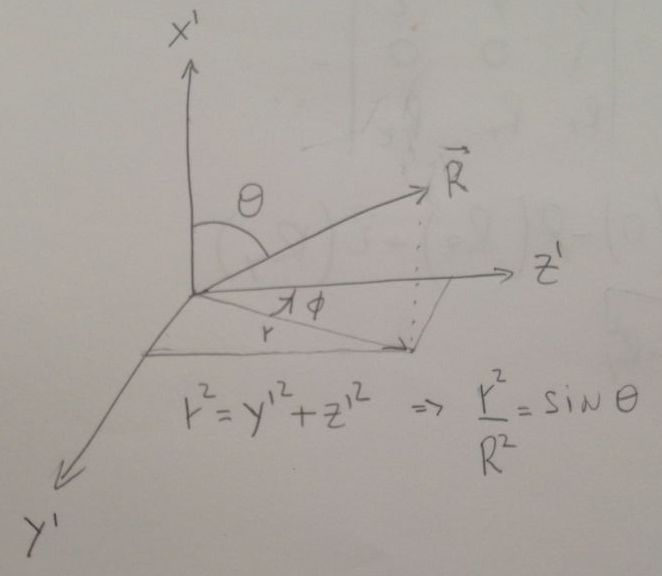
\includegraphics[width=0.7\textwidth]{L14_12}
    \caption{Coordinates scheme.}
    \label{fig:L14_12}
\end{figure}
Then, being \(\theta\) the angle between \(\vb{R}\) and \(\vu{x}\), we can use the figure \ref{fig:L14_12} to see that
\begin{equation}
    \vb{E}' = \frac{q}{4\pi \epsilon_0}\frac{\vb{R}}{R^3}\frac{\lr{1-\beta^2}}{\lr{1-\beta^2 \sin^2\theta}^{3/2}}
\end{equation}

Now, if \(\vb{B}_0 = 0\), we know that 
\begin{equation}
    \vb{B}' = - \frac{1}{c^2}\lr{\vb{v}_0}\cross \vb{E}' = \frac{1}{c^2}\lr{v_0}\vu{x}\cross \vb{E}'
\end{equation}

Also from figure \ref{fig:L14_12} we can see that \(\vu{x}\cross \vb{R} = \sqrt{R_y^2 + R_z^2}\vu{\phi}\), which leads to 
\begin{equation}
\begin{split}
    \vb{B}' &= \frac{\mu_0 q}{4\pi}\frac{\sqrt{R_y^2 + R_z^2}}{R}\frac{1}{R^2}\frac{\lr{1-\beta^2}}{\lr{1-\beta^2 \sin^2\theta}^{3/2}} v_0 \vu{\phi} \\
    &= \frac{\mu_0 q}{4\pi} \sin\theta \frac{\lr{1-\beta^2}}{\lr{1-\beta^2 \sin^2\theta}^{3/2}} \frac{v_0 \vu{\phi}}{R^2}  \\
    &= \frac{\mu_0}{4\pi} \frac{q v_0 \lr{1-\beta^2}\sin\theta}{\lr{1-\beta^2 \sin^2\theta}^{3/2}} \frac{\vu{\phi}}{R^2} 
\end{split}
\end{equation}


% \backmatter
% \printbib
\end{document}
	